% Add this once in the paper preamble:
% \usepackage{graphicx}
% \usepackage{tikz}
% \usetikzlibrary{arrows.meta,positioning,fit,calc,decorations.pathreplacing}
% \usepackage{tikz}
\usetikzlibrary{arrows.meta,positioning,fit,calc,decorations.pathreplacing}

\definecolor{icpaInk}{HTML}{1A1A1A}
\definecolor{icpaMuted}{HTML}{606A5B}
\definecolor{icpaLine}{HTML}{3F4A3A}
\definecolor{icpaSoftGray}{HTML}{F4F5F2}
\definecolor{icpaSoftGreen}{HTML}{E8F2E9}
\definecolor{icpaSoftBlue}{HTML}{EAF0F8}
\definecolor{icpaSoftGold}{HTML}{FFF6DD}
\definecolor{icpaSoftRose}{HTML}{FBEAEA}
\definecolor{icpaSoftViolet}{HTML}{F1ECF7}
\definecolor{icpaFuture}{HTML}{777777}

\tikzset{
  icpaBlock/.style={
    draw=icpaLine,
    rounded corners=2.2pt,
    line width=0.55pt,
    align=center,
    minimum height=9.4mm,
    inner sep=3.0pt,
    text=icpaInk,
    font=\sffamily\scriptsize
  },
  icpaSmall/.style={
    icpaBlock,
    minimum height=7.2mm,
    font=\sffamily\tiny
  },
  icpaGroup/.style={
    draw=icpaLine,
    rounded corners=3pt,
    line width=0.45pt,
    inner sep=4pt
  },
  icpaArrow/.style={
    -{Latex[length=2.0mm,width=1.25mm]},
    line width=0.55pt,
    draw=icpaLine
  },
  icpaDashed/.style={
    icpaArrow,
    dashed,
    draw=icpaFuture
  },
  icpaLabel/.style={
    font=\sffamily\tiny,
    text=icpaMuted,
    align=center
  },
  icpaLoss/.style={
    draw=icpaLine,
    rounded corners=1.8pt,
    line width=0.45pt,
    fill=white,
    align=left,
    font=\sffamily\tiny,
    inner sep=3pt,
    text=icpaInk
  }
}


\begin{figure*}[t]
  \centering
  \resizebox{\textwidth}{!}{%
    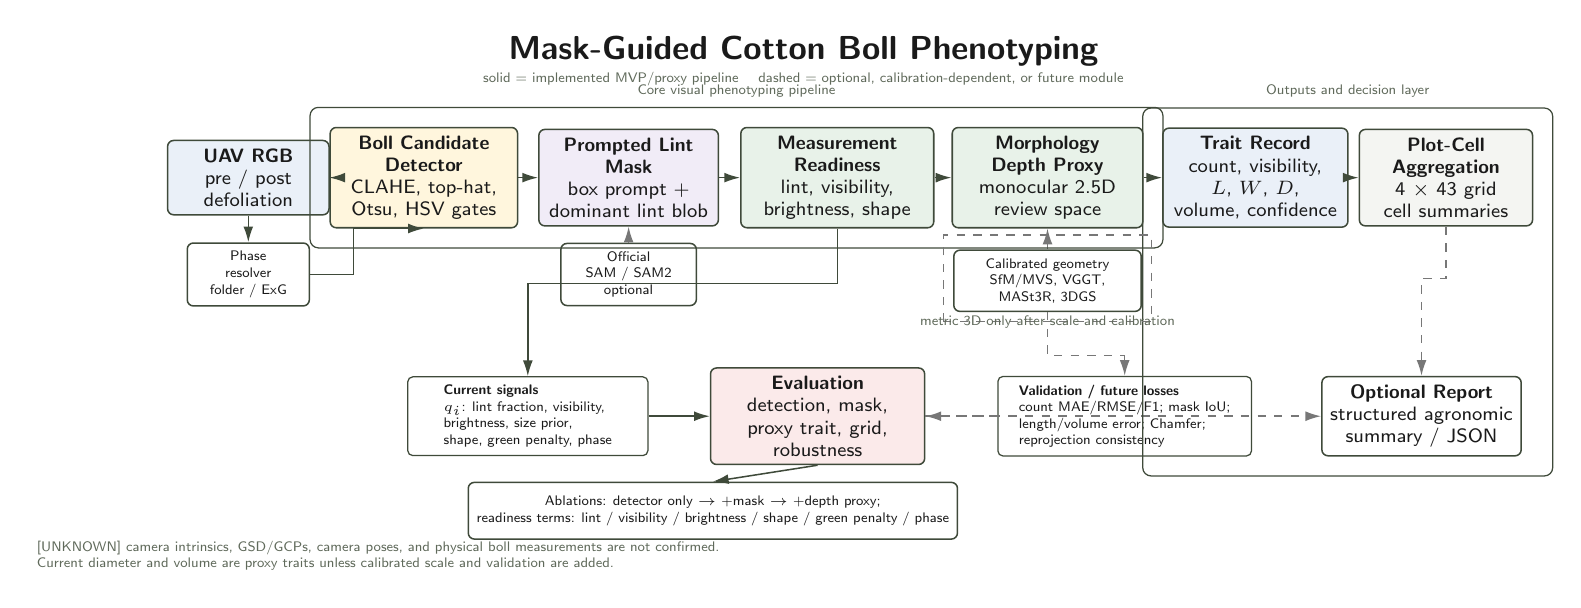
\begin{tikzpicture}[x=1cm,y=1cm]

\node[font=\sffamily\bfseries\large, text=icpaInk] at (8.0,6.45)
  {Mask-Guided Cotton Boll Phenotyping};
\node[font=\sffamily\tiny, text=icpaMuted] at (8.0,6.10)
  {solid = implemented MVP/proxy pipeline \quad dashed = optional, calibration-dependent, or future module};

% Main implemented pipeline.
\node[icpaBlock, fill=icpaSoftBlue, minimum width=2.05cm] (input) at (0.95,4.85)
  {\textbf{UAV RGB}\\pre / post\\defoliation};

\node[icpaSmall, fill=white, minimum width=1.55cm] (phase) at (0.95,3.62)
  {Phase\\resolver\\folder / ExG};
\draw[icpaArrow] (input) -- (phase);

\node[icpaBlock, fill=icpaSoftGold, minimum width=2.38cm] (detect) at (3.18,4.85)
  {\textbf{Boll Candidate}\\\textbf{Detector}\\CLAHE, top-hat,\\Otsu, HSV gates};
\draw[icpaArrow] (input.east) -- (detect.west);
\draw[icpaArrow] (phase.east) -- ++(0.55,0) |- (detect.south);

\node[icpaBlock, fill=icpaSoftViolet, minimum width=2.28cm] (mask) at (5.78,4.85)
  {\textbf{Prompted Lint}\\\textbf{Mask}\\box prompt +\\dominant lint blob};
\draw[icpaArrow] (detect.east) -- (mask.west);

\node[icpaSmall, fill=white, minimum width=1.72cm] (sam) at (5.78,3.62)
  {Official\\SAM / SAM2\\optional};
\draw[icpaDashed] (sam.north) -- (mask.south);

\node[icpaBlock, fill=icpaSoftGreen, minimum width=2.45cm] (quality) at (8.43,4.85)
  {\textbf{Measurement}\\\textbf{Readiness}\\lint, visibility,\\brightness, shape};
\draw[icpaArrow] (mask.east) -- (quality.west);

\node[icpaBlock, fill=icpaSoftGreen, minimum width=2.42cm] (depth) at (11.10,4.85)
  {\textbf{Morphology}\\\textbf{Depth Proxy}\\monocular 2.5D\\review space};
\draw[icpaArrow] (quality.east) -- (depth.west);

\node[icpaSmall, fill=white, minimum width=2.38cm] (calib) at (11.10,3.54)
  {Calibrated geometry\\SfM/MVS, VGGT,\\MASt3R, 3DGS};
\draw[icpaDashed] (calib.north) -- (depth.south);

\node[icpaBlock, fill=icpaSoftBlue, minimum width=2.35cm] (traits) at (13.74,4.85)
  {\textbf{Trait Record}\\count, visibility,\\$L$, $W$, $D$,\\volume, confidence};
\draw[icpaArrow] (depth.east) -- (traits.west);

\node[icpaBlock, fill=icpaSoftGray, minimum width=2.20cm] (grid) at (16.16,4.85)
  {\textbf{Plot-Cell}\\\textbf{Aggregation}\\4 $\times$ 43 grid\\cell summaries};
\draw[icpaArrow] (traits.east) -- (grid.west);

% Evaluation and signals.
\node[icpaLoss, minimum width=3.05cm] (signals) at (4.50,1.82)
  {\textbf{Current signals}\\
   $q_i$: lint fraction, visibility,\\
   brightness, size prior,\\
   shape, green penalty, phase};

\node[icpaBlock, fill=icpaSoftRose, minimum width=2.72cm] (eval) at (8.18,1.82)
  {\textbf{Evaluation}\\detection, mask,\\proxy trait, grid,\\robustness};

\node[icpaLoss, minimum width=3.22cm] (futureloss) at (12.08,1.82)
  {\textbf{Validation / future losses}\\
   count MAE/RMSE/F1; mask IoU;\\
   length/volume error; Chamfer;\\
   reprojection consistency};

\draw[icpaArrow] (quality.south) -- ++(0,-0.70) -| (signals.north);
\draw[icpaArrow] (signals.east) -- (eval.west);
\draw[icpaDashed] (calib.south) -- ++(0,-0.55) -| (futureloss.north);
\draw[icpaDashed] (futureloss.west) -- (eval.east);

\node[icpaBlock, fill=white, minimum width=2.52cm] (llm) at (15.85,1.82)
  {\textbf{Optional Report}\\structured agronomic\\summary / JSON};
\draw[icpaDashed] (grid.south) -- ++(0,-0.66) -| (llm.north);
\draw[icpaDashed] (eval.east) -- (llm.west);

% Grouping and notes.
\node[icpaGroup, fit=(detect)(mask)(quality)(depth), inner sep=7pt,
      label={[icpaLabel]above:Core visual phenotyping pipeline}] {};
\node[icpaGroup, fit=(traits)(grid)(llm), inner sep=7pt,
      label={[icpaLabel]above:Outputs and decision layer}] {};

\node[icpaSmall, fill=white, minimum width=5.20cm] (abl) at (6.85,0.62)
  {Ablations: detector only $\rightarrow$ +mask $\rightarrow$ +depth proxy;\\
   readiness terms: lint / visibility / brightness / shape / green penalty / phase};
\draw[icpaArrow] (eval.south) -- (abl.north);

\draw[dashed, line width=0.55pt, draw=icpaFuture] (9.78,3.02) rectangle (12.42,4.12);
\node[icpaLabel] at (11.10,3.02)
  {metric 3D only after scale and calibration};

\node[font=\sffamily\tiny, text=icpaMuted, align=left] at (2.60,0.05)
  {[UNKNOWN] camera intrinsics, GSD/GCPs, camera poses, and physical boll measurements are not confirmed.\\
   Current diameter and volume are proxy traits unless calibrated scale and validation are added.};

\end{tikzpicture}

  }
  \caption{\textbf{Mask-guided cotton boll phenotyping architecture.}
  UAV RGB frames acquired before and after defoliation are processed by a
  phase-aware detector that localizes bright lint candidates using illumination
  normalization, morphology, thresholding, and color gates. Candidate boxes
  prompt a SAM-style lint mask extractor, after which a measurement-readiness
  score combines lint fraction, visibility, brightness, shape, size, greenness,
  and phase cues. The current implementation projects selected evidence into a
  morphology-aware 2.5D review space and estimates proxy traits including count,
  length, width, diameter, volume, and confidence. Plot-cell aggregation
  summarizes records over the field grid. Solid arrows denote the implemented
  proxy pipeline; dashed arrows denote optional or calibration-dependent modules
  such as official SAM/SAM2, DINO-style features, SfM/MVS, DUSt3R/MASt3R/VGGT,
  and Gaussian Splatting. Metric 3D traits require camera calibration, scale
  information, and physical validation.}
  \label{fig:mask-guided-cotton-architecture}
\end{figure*}
